\documentclass[a4paper,10pt]{article}

\usepackage[margin=1in]{geometry} 	% Setea el margen manualmente, todos iguales.
\usepackage[spanish]{babel} 		% {Con estos dos anda
\usepackage[utf8]{inputenc} 		% todo lo que es tildes y ñ}
\usepackage{fancyhdr} 				%{Estos dos son para
\pagestyle{fancyplain} 				% el header copado}
\usepackage{color}					% Con esto puedo hacer la matufia de poner en color blanco un texto para engañar al formato
\usepackage{ulem}
\usepackage{caratula}
\usepackage{hyperref}

\lhead{Bases de Datos} 					% {Con esto se usa el header copado. También está \chead para
\rhead{Trabajo Práctico 2 - Grupo 8} 	% el centro y comandos para el pie de página, buscar fancyhdr}


%%%%%%%%%%%%%%%%%%%%%%%%%%%%%%%%%%%%%
%      COMANDOS ÚTILES USADOS       %
%%%%%%%%%%%%%%%%%%%%%%%%%%%%%%%%%%%%%

% \section{title} 		Te hace un título ``importante'' en negrita, numerado. También está \subsection{title} y \subsubsection{title}.
% \begin{itemize}		Te hace viñetas.
%	\item esto es un item	Cambiar itemize por enumerate te hace una numeración.
% \end{itemize}

% \textbf{text} 		Te hace el texto en negrita (bold).
% \underline{text}		Te subraya el texto.

% \textsuperscript{text}	Te hace ``superindices'' con texto. En teoría subscript debería funcionar, pero se puede usar guion bajo entre llaves
% 				y signos peso para hacerlo como alternativa. Sino buscar.

% \begin{tabular}{cols} 	Es para hacer tablas. Se pone una c por cada columna deseada dentro de cols (si es que se desea centrada, l para justificar a 
%	a & b & c		izquierda, r a la derecha). Si se separa por espacios la tabla no tendrá líneas divisorias. Si se separa por | en lugar de 
% \end{tabular}			espacios, aparecerá una línea. Con || dos, y así. Luego para los elementos de las filas se escriben y se separan con ampersand (&).
%				Finalmente, para las líneas horizontales, se usa \hline para una linea en toda la tabla y \cline{i - j} te hace la linea desde
%				la celda i hasta la j, arrancando en 1.
%				Si en la columna se pone p(width) podés escribir un párrafo en la celda. Para hacer un enter con \\ no funciona porque te hace un
%				enter en la fila. Para eso se usa el comando \newline.
  
% \textcolor{color predefinido en palabras}{text}

%%%%%%%%%%%%%%%%%%%%%%%%%%%%%%%%%%%%%
%    FIN COMANDOS ÚTILES USADOS     %
%%%%%%%%%%%%%%%%%%%%%%%%%%%%%%%%%%%%%

%%%%%%%
% Macros  %
%%%%%%%

% Tupla para hacer MR
% Uso: \tuple{NombreTabla}{Contenido de la tupla separado por comas}
% Pone en negrita el nombre de la tabla y envuelve en paréntesis el contenido. Recomiendo usar junto con \pk{} y \fk{} de ser necesario.
\newcommand{\tuple}[2]{\textbf{#1}(#2) \\}
% Primary key
% Uso: \pk{nombreDePK}
% Subraya la key.
\newcommand{\pk}[1]{\underline{#1}}
% Foreign key
% Uso: \fk{nombreDeFK}
% Subraya con línea punteada la key.
\newcommand{\fk}[1]{\dashuline{#1}}
% Restricción adicional
% Uso: \ra{Contenido de la restricción}
% Escribe "RA:" seguido de la restricción. Recomiendo usar junto con \attr{}.
\newcommand{\ra}[1]{RA: #1 \\}
% Atributo
% Uso: \attr{nombreDeAtributo}
% Pone al atributo en itálica.
\newcommand{\attr}[1]{\textit{#1}}
% Nota
% Uso: \nota{Contenido de la nota}
% Escribe "Nota:" seguido de la nota. Recomiendo usar junto con \attr{}.
\newcommand{\nota}[1]{\textit{Nota:} #1 \\}

%Datos para la caratula
\materia{Bases de Datos}

\titulo{Trabajo Práctico 2}

\integrante{García, Diego}{223/97}{diego.garcia.mail@gmail.com}
\integrante{Morales, Marcelino}{14/02}{marcelino.morales@gmail.com}
\integrante{Schmit, Matías}{714/11}{matias.schmit@gmail.com}
\integrante{Tastzian, Juan Manuel}{39/10}{jm@tast.com.ar}
\fecha{21 de Noviembre de 2015}

\begin{document}

\maketitle

\tableofcontents

\section{Introducción}
El objetivo de este trabajo práctico es tratar de modelar, de la manera más fiel posible, un problema del mundo real mediante un \textbf{Diagrama Entidad-Relación}(DER). Luego de tener determinado mediante dicho diagrama, las \textit{entidades}, sus \textit{atributos} e \textit{interrelaciones} entre ellas, se pasará a definir el \textbf{Modelo Relacional}.\\
\\
\indent El Modelo Relacional derivado del DER es el que representa fielmente el futuro modelado físico en una base de datos real. Este consta de \textbf{tuplas} que representan las \textbf{tablas} de la base de datos física, junto a sus \textbf{columnas}.\\
\\
\indent Las columnas en el modelo físico tendrán los nombres aquí expuestos, habiendo además, dos tipos especiales: las \pk{primary key} (clave primaria de la tabla, subrayada con línea sólida) y las \fk{foreign key} (subrayada con línea punteada, hace referencia a la primary key de otra tabla).\\
\\
\indent La estructura del trabajo práctico seguirá el órden que tomamos para el desarrollo de las distintas partes del mismo, es decir, primero el DER, luego el Modelo Relacional derivado, y finalmente tenemos aparte la base de datos física junto con las consultas pedidas en el enunciado.

\subsection{Datos de ejemplo}
Hemos buscado datos de ejemplo para agregarle un poco de realismo a las tablas y, en consecuencia, a los resultados de las consultas sobre la base de datos, y hemos encontrado las siguientes fuentes de información:
\begin{itemize}
	\item \href{https://www.sat.gob.pe/websitev8/Modulos/contenidos/mult_Papeletas_ti_rnt.aspx}{\textbf{Servicio de Administración Tributaria de Lima}} para los detalles de infracciones.
	\item \href{http://www.buenosaires.gob.ar/areas/obr_publicas/lic_conducir/categorias.php?menu_id=6427}{\textbf{Categorías de licencias de conducir de la Ciudad de Buenos Aires}}.
\end{itemize}

\section{Desnormalizaci\'on}

Para la resoluci\'on de este ejercicio entregamos el dise\~no f\'isico de la DB realizado en formato JSON con el agregado de que en lugar de indicar un valor para cada atributo indicamos el tipo de datos. De esta forma hacemos mas legible el modelo. Adem\'as discutimos cada uno de los puntos de optimizaci\'on pedidos comentando las distintas variantes que evaluamos para la resoluci\'on de los mismos. Para la definici\'on de los tipos de datos a utilizar, al no estar especificados en el DER, los elegimos de la forma que nos pareci\'o mas relevante al contexto.

El dise\~no de la DB propuesto es el siguiente:
   
\begin{verbatim}
db: {
	Clientes: [{
		DNI						: int,
		Nombre					: string,
		Edad					: int,
		CantCompras				: int,
		CantComprasMismaEdad	: int
	}], 
	Empleados: [{
		NroLegajo,
		Nombre,
		ClientesAtendidos:[{ 
			DNI		: int, 
			Edad	: int,
			Nombre	: string,
			Fecha	: string
		}],
		Sectores: [{
			CodSector: string,
			IdTarea: int
		}]
	}],
	Articulos: [{
		CodBarras	: string,
		Nombre		: string,
		CantVendidos: int,
		CodSector	: string
	}],
	Sectores: [{
		CodSector: string,
		Trabaja: [{
			NroLegajo, 
			IdTarea
		}]
	}],
	Tareas: [{
		IdTarea: int,
		Descripcion: string
	}]
}
\end{verbatim}

\subsection{Resoluci\'on de Consultas}

\subsubsection{Empleados que atendieron a clientes de mayor edad}

Para resolver esta consulta embebimos informaci\'on de los clientes dentro del documento de Empleados, agregando una lista de clientes atendidos. De esta forma, al obtener el documento del empleado correspondiente podemos acceder directamente a los datos de todos los clientes que fueron atendidos por \'el, y por lo tanto tambi\'en podemos hacer un filtro sobre la entidad Empleados que devuelva los empleados que atendieron a los clientes mayores de edad.

\subsubsection{Los articulos mas vendidos}

Para resolver esta consulta se nos ocurren 3 opciones:

\begin{enumerate}
	\item Embeber la informaci\'on de compra dentro del art\'iculo. El problema con este enfoque es que se replicar\'ia la informaci\'on del cliente en cada compra, y adem\'as la consulta pedida queda muy compleja de hacer.

	\item Mantener una lista de art\'iculos comprados dentro de cada cliente. Esto reduce la replicaci\'on de informaci\'on, pero sigue sin solucionar la complejidad de la consulta pedida.

	\item Finalmente, optamos por reutilizar la idea del punto 2 y agregar un contador de ventas dentro de cada art\'iculo. Esto nos permite resolver la consulta de manera eficiente, con m\'inima redundancia, sin perder la informaci\'on del modelo.
\end{enumerate}

\subsubsection{Los sectores donde trabajan exactamente 3 empleados}

La consulta se resuelve buscando qu\'e sectores tienen exactamente 3 elementos en el array "Trabaja". Esto vale porque la aridad de la ternaria no permite que haya un empleado de un sector con m\'as de 1 tarea asignada

Para resolver esta consulta embebimos una parte de la informaci\'on perteneciente a la entidad Empleado dentro del documento Sector, de esta forma resolvemos efici\'entemente la consulta (que se realiza contando la cantidad de elementos del array Trabajapor cada sector) y mantenemos replicada solo la informaci\'on necesaria para resolverla.

\subsubsection{El empleado que trabaja en m\'as sectores}

Para esta consulta decicimos guardar en cada empleado una lista de los sectores en los que trabaja. De esta forma podemos resolver esta consulta contando la longitud del array de sectores de cada empleado, y qued\'andonos con el de mayor longitud. 

\subsubsection{Ranking de los clientes con mayor cantidad de compras}

Para optimizar al m\'aximo esta consulta optamos por mantener un contador de compras dentro del documento de clientes. De esta forma resulta trivial el armado de un ranking de clientes con mayor cantidad de compras. Adem\'as esta opci\'on solo requiere que al realizar una venta actualicemos el contador de compras del cliente.

\subsubsection{Cantidad de compras realizadas por clientes de la misma edad}

Para resolver esta consulta decidimos agregar un contador de compras extra a la entidad cliente que cuenta el n\'umero de compras realizadas por clientes de esa edad. De esta forma por cada compra realizada, debemos incrementar el contador de todos los clientes que tengan la misma edad que el contador. \'Esto nos permite mantener un nivel \'optimo de redundancia y evitar soluciones mas desprolijas como crear una tabla de edades por ejemplo.



\section{Map Reduce}


\section{Sharding}


\subsection{Funcion de creación de datos}
Se utilizo el siguiente código en js, para generar las inserciones de datos, permitiendo definir un total y un tamaño de lote (y una pausa si fuera necesario). La función genera registros para insertar,en este caso únicamente con código postal aleatorio (ya que era lo importante para el ejemplo) e imprime la información provista por los comandos que provee mongodb para reportar el estado del sharding 	\textbf{sh.status()} y \textbf{db.collection.getShardDistribution()}.

\begin{lstlisting}
function insertRandomPersonas(total, tam_intervalo, pausa_seg) {

	var start = new Date().getTime();
	var total_count = total;
	
	var cp_size = 99999 ;
	print ("Inicial");
	sh.status()
	db.personas.getShardDistribution()
	print ("------------------------------------------------------------------------");
	
	while (total_count>0){
		var current_loop = Math.min(total_count, tam_intervalo);
		for (var i = 1; i <= current_loop; i++) {
			
			var randomCP = Math.floor((Math.random() * cp_size) );
		
			db.personas.insert({"nombre" : "Juan Perez" ,"password" : "1234" ,"codigo_postal" : randomCP  ,"genero" : "m" ,	"edad" : 28 ,	"fecha_creacion": "2015-01-01"} )
		}
		total_count = total_count - current_loop;
		var end = new Date().getTime();
		var time = end - start;
		print ("Restantes:"+total_count+" Execution time: " + time);
		sh.status()
		db.personas.getShardDistribution()
		print ("------------------------------------------------------------------------");
		sleep(pausa_seg * 1000);
	}
}
\end{lstlisting}

La llamada para insertar 5000000 registros en rangos de 20000 es la siguiente: 
\begin{lstlisting}
insertRandomPersonas(500000,20000,0);
\end{lstlisting}

\subsection{Pruebas}
Para las pruebas a realizar se configuraron 4 shards de acuerdo al tutorial provisto por la cátedra y se realizaron pruebas primero utilizando un \textit{indice simple} y después (regenerando de cero los shards) un \textit{indice hash}.\\
Se realizaron varias pruebas para cada tipo de indice, sin embargo se provee solo un ejemplo de cada una, ya que los resultados por tipo de indice tuvieron el mismo comportamiento, sin tener exactamente las mismas cantidades insertadas por el componente aleatorio en la insercion. 

\pagebreak

\subsection{Resultados}
\textbf{Indice Simple} \\
\begin{tabular}{ | l | l | l | l | l | }
\hline
	Cant Registros Insertados & Shard1 & Shard2 & Shard3 & Shard4 \\ \hline
	0 & 0 & 0 & 0 & 0 \\ \hline
	20000 & 3441 & 8237 & 8322 & 0 \\ \hline
	40000 & 6925 & 16346 & 16729 & 0 \\ \hline
	60000 & 10362 & 24416 & 25222 & 0 \\ \hline
	80000 & 13829 & 32392 & 33779 & 0 \\ \hline
	100000 & 17128 & 40546 & 42326 & 0 \\ \hline
	120000 & 20478 & 48579 & 50943 & 0 \\ \hline
	140000 & 23888 & 56671 & 59441 & 0 \\ \hline
	160000 & 27289 & 64815 & 67896 & 0 \\ \hline
	180000 & 30705 & 72895 & 38764 & 37636 \\ \hline
	200000 & 34168 & 80927 & 43157 & 41748 \\ \hline
	220000 & 37626 & 88957 & 47486 & 45931 \\ \hline
	240000 & 41100 & 97070 & 51754 & 50076 \\ \hline
	260000 & 44453 & 66860 & 56108 & 92579 \\ \hline
	280000 & 47847 & 72029 & 60453 & 99671 \\ \hline
	300000 & 51300 & 77048 & 64775 & 106877 \\ \hline
	320000 & 54697 & 82171 & 69025 & 114107 \\ \hline
	340000 & 58072 & 87357 & 73420 & 121151 \\ \hline
	360000 & 61526 & 92442 & 77729 & 128303 \\ \hline
	380000 & 65013 & 97555 & 82002 & 135430 \\ \hline
	400000 & 68423 & 102615 & 86393 & 142569 \\ \hline
	420000 & 108673 & 107816 & 53816 & 149695 \\ \hline
	440000 & 113798 & 112928 & 56349 & 156925 \\ \hline
	460000 & 119068 & 117956 & 58953 & 164023 \\ \hline
	480000 & 124353 & 122915 & 61521 & 171211 \\ \hline
	500000 & 129591 & 127964 & 64092 & 178353 \\ \hline
\end{tabular} \\
 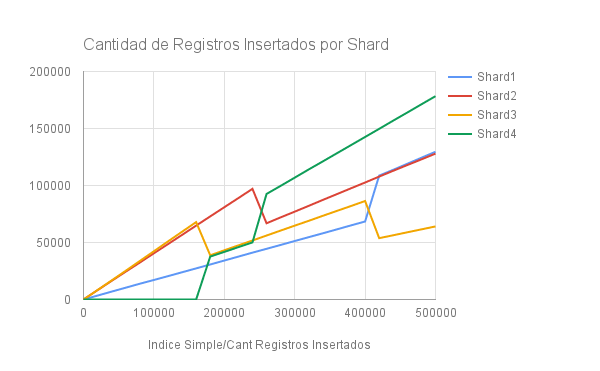
\includegraphics[width=\linewidth]{IndiceSimpleChart.png}
\pagebreak

\textbf{Indice Hash} \\
\begin{tabular}{ | l | l | l | l | l | }
\hline
	Cant Registros Insertados & Shard1 & Shard2 & Shard3 & Shard4 \\ \hline
	0 & 0 & 0 & 0 & 0 \\ \hline
	20000 & 5039 & 4901 & 5067 & 4993 \\ \hline
	40000 & 10170 & 9942 & 9967 & 9921 \\ \hline
	60000 & 15211 & 14962 & 15003 & 14824 \\ \hline
	80000 & 20109 & 20089 & 19971 & 19831 \\ \hline
	100000 & 25155 & 25113 & 24940 & 24792 \\ \hline
	120000 & 30143 & 30194 & 29923 & 29740 \\ \hline
	140000 & 35116 & 35160 & 34950 & 34774 \\ \hline
	160000 & 40093 & 40220 & 39926 & 39761 \\ \hline
	180000 & 45084 & 45172 & 44947 & 44797 \\ \hline
	200000 & 50160 & 50210 & 49953 & 49677 \\ \hline
	220000 & 55212 & 55214 & 54972 & 54602 \\ \hline
	240000 & 60194 & 60226 & 59949 & 59631 \\ \hline
	260000 & 65222 & 65226 & 64931 & 64621 \\ \hline
	280000 & 70210 & 70247 & 69921 & 69622 \\ \hline
	300000 & 75309 & 75162 & 74942 & 74587 \\ \hline
	320000 & 80403 & 80062 & 80020 & 79515 \\ \hline
	340000 & 85527 & 84939 & 84987 & 84547 \\ \hline
	360000 & 90583 & 89902 & 89914 & 89601 \\ \hline
	380000 & 95566 & 94898 & 94837 & 94699 \\ \hline
	400000 & 100428 & 99931 & 99805 & 99836 \\ \hline
	420000 & 105363 & 105137 & 104749 & 104751 \\ \hline
	440000 & 110394 & 110037 & 109801 & 109768 \\ \hline
	460000 & 115318 & 115106 & 114785 & 114791 \\ \hline
	480000 & 120196 & 120176 & 119788 & 119840 \\ \hline
	500000 & 125288 & 125160 & 124708 & 124844 \\ \hline
\end{tabular} \\
 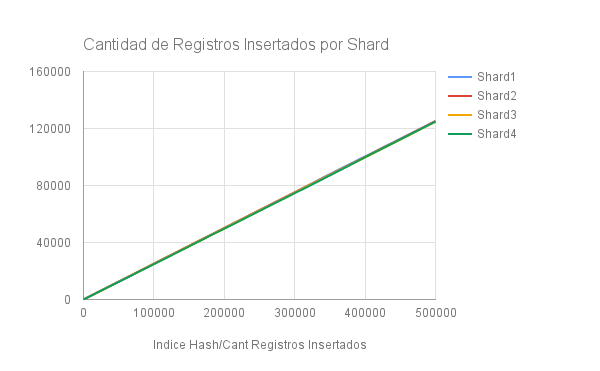
\includegraphics[width=\linewidth]{IndiceHashChart.png}
 
\pagebreak
\subsection{Análisis}

Se puede ver que  utilizando un \textit{indice simple} para un campo en el cual los datos estan generados de manera aleatoria, lo que sucede es que empieza a crecer un shard mas que otros y en algun momento el balanceador decide migrar un subconjunto de estos datos a otro shard menos cargado. Esto se va realizando varias veces durante la carga de datos, de acuerdo al nivel de crecimiento de cada shard.\\
Una vez realizadas las pruebas verificamos cual es el mecanismo utilizado por mongodb en estos casos y esta explicado en la seccion \textbf{Chunk Migration Across Shards} del manual de mongodb. Básicamente decide balancear cuando la diferencia entre la cantidad de \textit{chunks} entre el shard con mas \textit{chunks}  y el shard con menos \textit{chunks} es superior a un valor configurado internamente dentro del balanceador de mongodb.\\
Utilizando un \textit{indice hash} lo que sucede es que los registros generados se van insertando de manera pareja entre todos los shards y en ese caso nunca le hace falta al balanceador hacer una migración de \textit{chunks}.

\subsection{Escenarios posibles para sharding}
Algunos escenarios posibles para sharding son:\\

Tener una base con consultas/visitas de clientes a un sitio web con alta concurrencia, que guarden que items vio, en que esta interesado, historial de navegación, etc. Estas consultas/visitas pueden crecer muy rápidamente y generar un volumen my grande de datos. En este caso una base con mongodb con sharding permitiría un crecimiento acorde al uso que va teniendo la aplicación.Un atributo posible para sharding en este caso es el numero de cliente.\\

Tener una empresa de logística o correo, que quiere mantener una base con el total de envíos de paquetes realizados, en este caso se podría utilizar como atributo de sharding código postal del destinatario, siempre y cuando el envío de paquetes realizados tenga una distribución uniforme ( o lo mas próxima posible a uniforme ) y variada de destinos para los envíos con los que trabaja.En este caso la base podría crecer lo que fuera necesario y sabríamos que tendríamos equilibrada entre todos los shards.\\

Queremos tener una base de datos de usuarios conectados a un juego online de alta concurrencia. Esta base debe guardar información variada de los jugadores y de las partidas mientras están conectados. Esta base puede tener variaciones en la carga dependiendo de los días del horario, día de la semana o época del año (en vacaciones tiene mas uso). En este caso se podría usar el sharding para permitir un crecimiento/decrecimiento de la base de acuerdo a lo que fuera necesario y de manera equilibrada. En este caso podríamos usar como atributo para sharding el id de jugador.\\


\subsection{Características de un atributo para sharding}
Un atributo para ser usado como clave en un esquema de sharding debe tener algunas características:\\

\begin{itemize}		
	\item Alta Cardinalidad: Si un atributo tiene baja cardinalidad no es útil para sharding, ya que todos los registros con el mismo atributo terminan en un mismo chunk y en caso de que uno quisiera tener un numero grande de shards, esta acotado por la cardinalidad de este atributo.
	\item Tener una distribución uniforme: Un atributo debe tener una distribucion uniforme para el dominio del problema en el que se esta trabajando, ya que si no es posible que se llenen mucho algunos shards y otros queden vacios. Por ejemplo utilizar código postal como clave para shard puede ser bueno (inclusive con los balanceos) si tiene una distribución pareja (tenemos personas o clientes de todo el país), sin embargo si nuestra base de clientes es de un solo barrio de una ciudad, la variabilidad de códigos postales puede ser muy acotada.
\end{itemize}


\section{Otras bases de datos NoSQL}


\section{Conclusiones}

Este trabajo nos permiti\'o poner en pr\'actica muchos de los conocimientos vistos en clase sobre bases de datos no relacionales y realizar una implementaci\'on concreta sobre el motor DB Mongo. De esta forma, nos concentramos en la utilizaci\'on de un tipo de bases de datos en particular, pero tambi\'en evaluamos en forma mas general otros tipos de bases de datos.


\end{document}
%\section{Sección, título grande}
%\\
%\textcolor{white}{Sarasa engañadora de formato, jua jua}
%Esto es texto. Con doble barra invertida es el enter.
%\\
%\\
%\textit{De acá en adelante, todo lo que se explica como "para hacer x se usa y", implica que antes de y va una barra invertida}
%\\
%\\
%Con \textbf{textbf\{\}} se escribe en negrita.
%\\
%\\
%\section{Bullet \& Numbering}
%Para hacer items se usa \textbf{begin\{itemize\}} y \textbf{end\{itemize\}}, por ejemplo:
%\begin{itemize}
%	\item Esto es un ítem.
%	\item Esto es otro.
%\end{itemize}
%Con \textbf{item} se hace cada uno de los ítems. Si cambiás \textbf{itemize} por \textbf{enumerate} te lo hace enumerado. Por ejemplo:
%\begin{enumerate}
%	\item Acá está el primero.
%	\item Acá el segundo.
%\end{enumerate}
%\\
%Y así.
%\\
%\\
%\section{Tablas}
%También tenemos las tablas, que son un poco más rebuscadas. Se usa \textbf{begin\{tabular\}\{cols\}} y en cols ponemos c si queremos una columna centrada, l y r
%para otro tipo de justificación. Si las c las separás con espacios, se hacen columnas sin división. Si ponés un pipe es con una línea divisoria, dos pipes con
%dos líneas, y así. Se termina con \textbf{end\{tabular\}}. Para separar entre elementos de fila/columna se usa un ampersand (\&, y es necesario para separar
%elementos entre filas y columnas, no solo entre filas) y para cambiar de fila \textbf{SIN} linea divisoria, un \textbf{newline} ya que el doble barra invertida
%te hace un enter dentro de la celda. Con línea divisoria es reemplazando \textbf{newline} por \textbf{hline}.
%\\
%\\
%Más datos en el principio de este tex. Un ejemplo:
%\\
%\\
%\begin{tabular}{| c| c|}\hline
%    Celda 1 & Celda 2 &\hline
%    Celda 3 & Celda 4 &\hline
%\end{tabular}
%\\
%\\
%\section{Verbatim}
%\begin{verbatim}
%Esto es verbatim. Es un entorno que no le da ni 5 de pelota al formato de latex.
%Por eso mismo hay que tener cuidado con no irse de la hoja o similar.
%Sirve por ejemplo, para pseudocódigo:
%
%if (se cumple sarasa){
%    ejecuto cosito1;
%    ejecuto cosito2:
%}else{
%    ejecuto cosito3:
%}
%\end{verbatim}
%
%
%\end{document}